\documentclass[pdftex,12pt,a4paper]{article}

\usepackage{graphicx}  
\usepackage[margin=2.5cm]{geometry}
\usepackage{breakcites}
\usepackage{indentfirst}
\usepackage{pgfgantt}
\usepackage{pdflscape}
\usepackage{float}
\usepackage{epsfig}
\usepackage{epstopdf}
\usepackage[cmex10]{amsmath}
\usepackage{stfloats}
\usepackage{multirow}

\renewcommand{\refname}{REFERENCES}
\linespread{1.3}

\usepackage{mathtools}
%\newcommand{\HRule}{\rule{\linewidth}{0.5mm}}
\thispagestyle{empty}
\begin{document}
\begin{titlepage}
\begin{center}
\textbf{}\\
\textbf{\Large{ISTANBUL TECHNICAL UNIVERSITY}}\\
\vspace{0.5cm}
\textbf{\Large{COMPUTER ENGINEERING DEPARTMENT}}\\
\vspace{2cm}
\textbf{\Large{BLG 242E\\ DIGITAL CIRCUITS LABORATORY\\ HOMEWORK 1}}\\
\vspace{2.8cm}
\begin{table}[ht]
\centering
\Large{
\begin{tabular}{lcl}
\textbf{HOMEWORK NO}  & : & 1 \\
\textbf{HOMEWORK DATE}  & : & 20.03.2023\\
\textbf{LAB SESSION}  & : & FRIDAY - 10.30 \\
\textbf{GROUP NO}  & : & G8 \\
\end{tabular}}
\end{table}
\vspace{1cm}
\textbf{\Large{GROUP MEMBERS:}}\\
\begin{table}[ht]
\centering
\Large{
\begin{tabular}{rcl}
150200919  & : & Abdullah Jafar Mansour Shamout \\
150220762  & : & Muhammed Yusuf Mermer  \\
\end{tabular}}
\end{table}
\vspace{2.8cm}
\textbf{\Large{SPRING 2023}}

\end{center}

\end{titlepage}

\thispagestyle{empty}
\addtocontents{toc}{\contentsline {section}{\numberline {}FRONT COVER}{}}
\addtocontents{toc}{\contentsline {section}{\numberline {}CONTENTS}{}}
\setcounter{tocdepth}{4}
\tableofcontents
\clearpage

\setcounter{page}{1}

\section{INTRODUCTION}
In this experiment we implemented combinational logic circuits and Full adder
using the Verilog. In it we learned how to design and use a module. We found the minimal cost expression using prime implicants method and prime implicants chart then using our basic logic gates that we designed, we implemented the modules. We also recalled the signed and unsigned addition and subtraction using 2's complement, this helped us in implementing adders and subtractors using combinational logic circuits modules. Through out our designs and implementations, we made sure to test all of our modules with various inputs through simulations with different combinations to make sure they work properly.

\section{PRELIMINARY}

\subsection{Question 1.a)}

To find with K-Map, at first we find prime implicant for implicants.

Prime implicant is biggest implicants for that group of 1's.

   \begin{figure}[H]
    	\centering
    	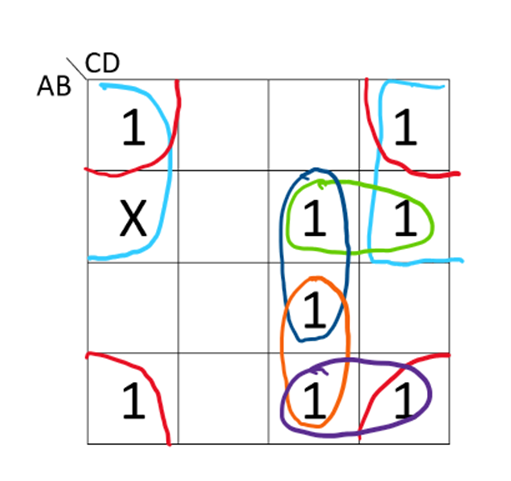
\includegraphics[width=0.8\textwidth]{preliminary/kmap_at_first.png}	
    	\caption{K-Map With All Prime Implicants}
    	\label{K-Map With All Prime Implicants}
    \end{figure}
    

 Then, to find essential prime implicants, we need to take prime implicants who are just covered by one and only one prime implicants.

After that, make other prime implicants with remaing 1's. Try to prevent collisions and make prime implicant big as possible. 

   \begin{figure}[H]
    	\centering
    	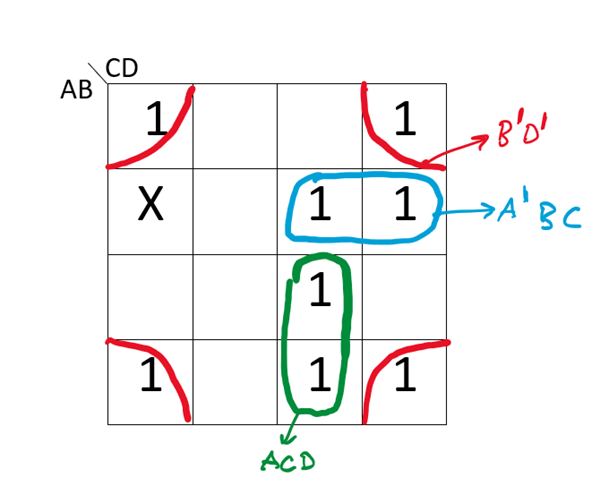
\includegraphics[width=0.8\textwidth]{preliminary/kmap_last.png}	
    	\caption{at end of the K-Map}
    	\label{at end of the K-Map}
    \end{figure}
    
 \begin{center} \textbf{$acd+a'bc+b'd'$ will be the final result.}
\end{center}


\subsection{Question 1.b)}
To find with Quine Mccluskey method, at first we need to write all implicants(including don't care condition) to table (like binary digits) as in the figure:
   \begin{figure}[H]
    	\centering
    	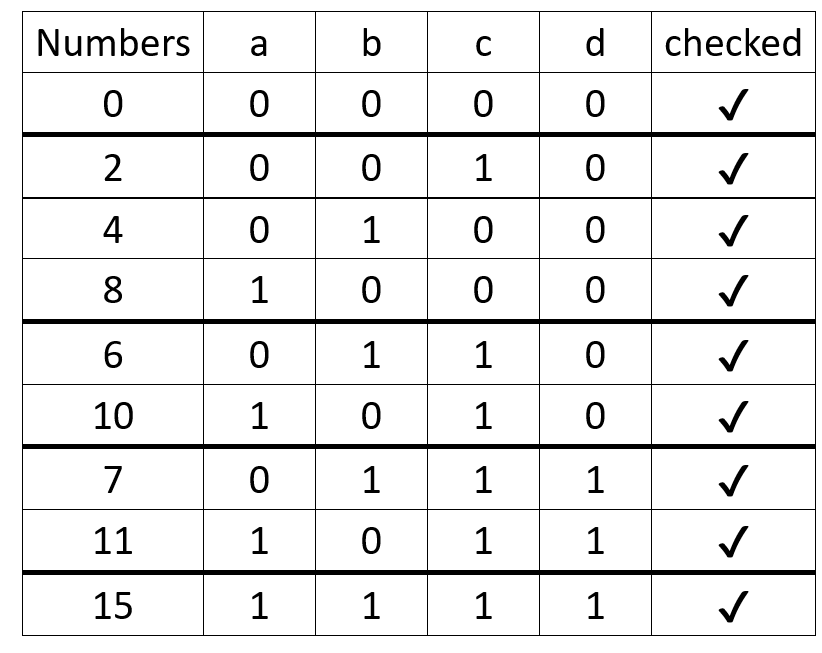
\includegraphics[width=0.8\textwidth]{preliminary/input_combinations.png}	
    	\caption{input combinations}
    	\label{input combinations}
    \end{figure}

After this operation, we made pairs from different groups which have only one digit difference. And we checked previous rows if they are used in new table:


   \begin{figure}[H]
    	\centering
    	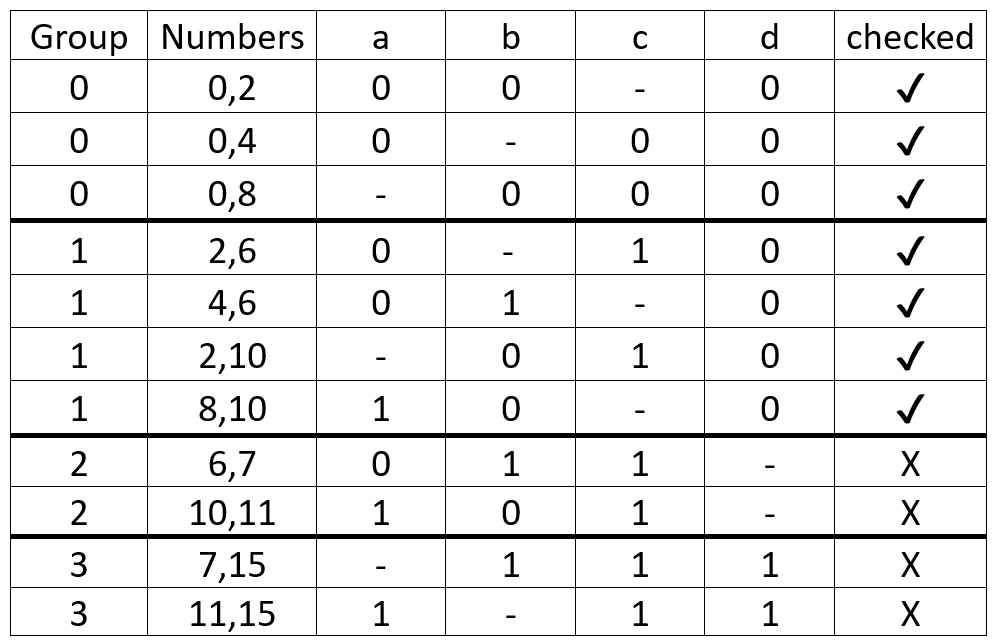
\includegraphics[width=0.8\textwidth]{preliminary/group_of_two.png}	
    	\caption{Group with 2 points}
    	\label{Group with 2 points}
    \end{figure}

Do same things for group of 4's: 
   \begin{figure}[H]
    	\centering
    	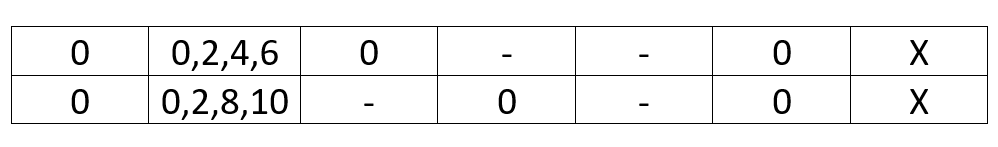
\includegraphics[width=0.8\textwidth]{preliminary/group_of_four.png}	
    	\caption{Group with 4 points}
    	\label{Group with 4 points}
    \end{figure}

    
\subsection{Question 1.c)}

    To find cost, we used unchecked  rows. We didn't include the don't care conditions but we used them to calculate costs. As it mentioned in the question, 2 cost for variables and 1 more cost for their inverts used to calculate over all cost.
   \begin{figure}[H]
    	\centering
    	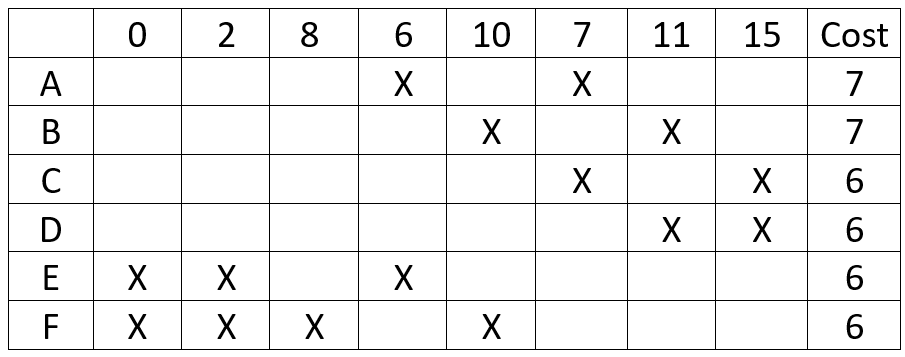
\includegraphics[width=0.8\textwidth]{preliminary/true_points.png}	
    	\caption{True Points of The Function}
    	\label{True Points of The Function}
    \end{figure}

For the simplification, we need to find distinguished points. Distinguished points' column doesn't have any more X's.

   \begin{figure}[H]
    	\centering
    	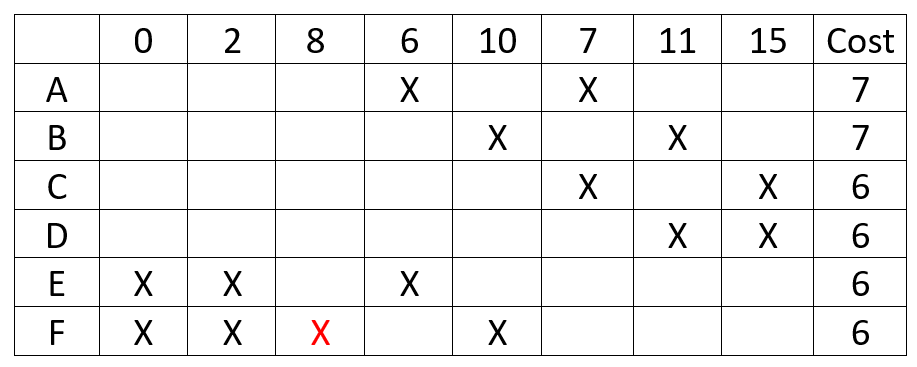
\includegraphics[width=0.8\textwidth]{preliminary/distinguished_point.png}	
    	\caption{Distinguished Points}
    	\label{Distinguished Points}
    \end{figure}

    Then we deleted the row F but we will use it for the overall cost calculation. Not only row F, but we also deleted columns which are covered by the F.

   \begin{figure}[H]
    	\centering
    	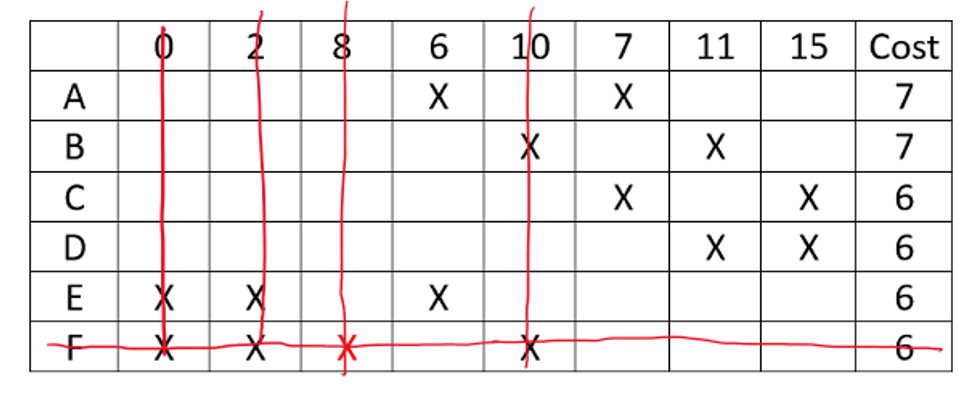
\includegraphics[width=0.8\textwidth]{preliminary/simplification_of_chart.png}	
    	\caption{Simplification of Chart}
    	\label{Simplification of Chart}
    \end{figure}

In here, it is better to delete row B as \textbf{D $<$ B $+$ one more variable}.
Do the same thing for E. row. 
    
   \begin{figure}[H]
    	\centering
    	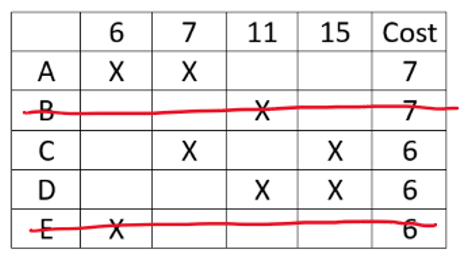
\includegraphics[width=0.8\textwidth]{preliminary/last_simplification.png}	
    	\caption{Last Simplification}
    	\label{Last Simplification}
    \end{figure}

At the end, we will look distinguished points again. This time both A and D are distinguished points.

   \begin{figure}[H]
    	\centering
    	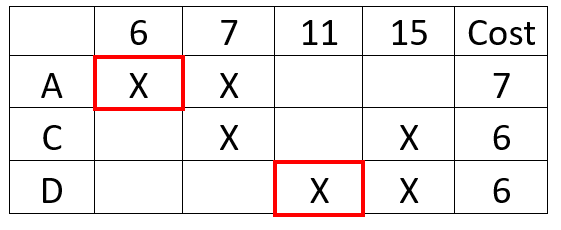
\includegraphics[width=0.8\textwidth]{preliminary/last_two_distinguish_points.png}	
    	\caption{Selecting Last Distinguished Points}
    	\label{Selecting Last Distinguished Points}
    \end{figure}

\begin{center}
    Result will be \textbf{$F+A+D=6+7+6=19$}
\end{center}
\subsection{Question 1.d and 1.e)}

After designing circuit with AND, OR, NOT gates, to convert equation to NAND gate, we take the NOT of whole equation and also to maintain accuracy, we distributed inverse to inside of the equation. Therefore, OR gate turned into AND gate. 

\begin{center} $((acd)' \& (a'bc)' \& (b'd')')'$ \end{center}
Prime implicants already in AND form, so without distributing even more we can take their inverses to obtain NAND gates from them.

Circuit designs implemented in Figure 29 and 31.


\subsection{Question 1.f)}

Multiplexer has 3 selector. We can give a b c variables to this selectors. Then as a inputs of MUX, we can give d, d', 0 or 1  according to a, b, c values in the truth table.

   \begin{figure}[H]
    	\centering
    	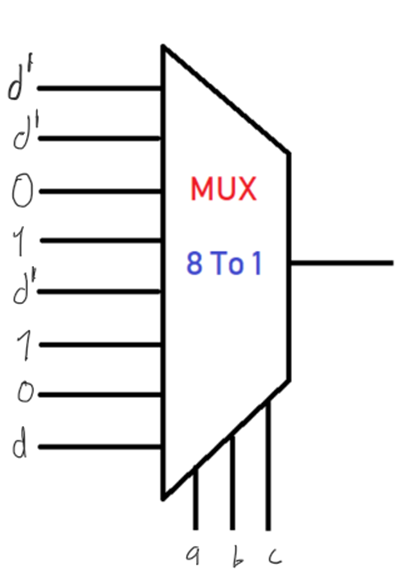
\includegraphics[width=0.4\textwidth]{preliminary/mux_prelim_1.png}	
    	\caption{MUX 8x1}
    	\label{MUX 8x1}
    \end{figure}

 The circuit design implemented in Figure 33.

\subsection{Question 2)}
Using a decoder, we were able to create all possible minterms for (a,b,c), after that by using OR gates we where able to join them together to create the requested expressions, for F3 we also used our knowledge of boolean algebra to get rid of the (c) variable in the minterm.
    
\subsection{Question 3)}
    \subsubsection{Signed and Unsigned Addition For Binary Numbers}
    For adding two binary numbers we start form LSB (Least significant bit). Using logic, 0 and 0 results in a 0, 1 and 0 results in 1, 1 and 1 results in a carry to the bit more significant that it by 1.
    After we continue to the next left bit, after we make the addition we add the carry value to the result. For two n-bit unsigned integers added there can be a resultant carry needing a (n+1)th bit. This results in no problems if we use n+1 bits to represent the number, or else we cant represent it.
    For n-bit signed integers, its the same as unsigned integers, however, their MSB represents the sign, and bits greater than the nth bit (n+1) are ignored. If a carry occurs there could be an overflow.it happens when we add two positive numbers and get a negative number, or when we add two negative numbers and get a positive one.
    
    \subsubsection{Signed and Unsigned Subtraction For Binary Numbers}
    In binary we do not use subtraction directly, we change the second operand to its negative value and add it to the first one, which is the same as subtraction. For that we use 2's complement: Flip all 1's and 0's to their counterpart, then add 1 to that value, this way we achieved that number's 2's complement. Then we add both numbers. For unsigned integer subtraction we can get either a carry or a borrow, if we get a carry then we just ignore it and the result is valid, if we get a borrow "no carry" then the result is invalid and the number can not be represented. For signed integer subtraction however,if there is a carry we just ignore it, but we need to check for the sign bits as an overflow can also occur here. if we have a negative - positive and get positive or if we have positive - negative and get negative then these are cases of overflow and we cannot represent them.
    
\section{EXPERIMENT}

\subsection{Part 1}

\begin{itemize}
\item To develop AND we used the bitwise operator \&
we created a normal 2-input AND module, a 3-input AND module for the 3 to 8 decoder, a 4-input AND module for the 8:1 multiplexer. 
\item To develop OR we used the bitwise operator \textbar
we created a normal 2-input OR module, an 8-input OR module for the 8:1 multiplexer.
\item To develop NOT we used the bitwise operator \~ ~ 
we developed a normal 1-input NOT module.
\item To develop a XOR module we could not use its bitwise operator according to the question, so we had to develop it from its expression A'B + AB', thus we used two NOT gates to inverse A and B we also used two AND gates to join A' with B and A with B' the used an OR module to join the two terms to create an XOR.
\item To develop a NAND module we used a normal 2-input AND gate and complemented its output to get a NAND.
\item To develop a 8:1 MUX module we need three selector inputs s1-s3, then to create combinations from them we took the complement of each of these selectors. Then we utilized our 4 input AND modules each would take a unique combination of the 3 selectors and a unique input from 1 to 8. Then all the outputs of the AND modules were (OR)ed using our 8 input or module, since with the selectors only 1 and gate could give an output so to take that output we OR all of them to get our value from the MUX.
\item To develop a 3:8 decoder, we need 3 inputs, we also invert those inputs to be able to enumerate 8 values of output. Then we use three input AND modules to AND unique combinations of the 3 inputs to get a unique output from each AND module, thus creating 8 outputs.
\end{itemize}

\subsection{Part 2}
We used 4 wires for inputs. 8 wires used as intermediate section. Then, with the help of NOT modules, we inverted input $a$, $b$ and $d$, and stored them in 3 intermediate wires. First $a' \& b$ calculated with AND gate. Again with AND gate result multiplied with $c$ to get $a'bc$. For the second prime implicant, we multiplied $a$ and $c$ with AND module. Their result multiplied by $d$ via AND gate to find $acd$. We store information in each step in different intermediate wires. At the end, $b'$ and $d'$ multiplied by AND gate. $a'bc$, $acd$, $b'd'$ prime implicants summed using 3 input OR gates. To verify our results we also ran simulations with different inputs.


\subsection{Part 3}

With the same 4 inputs, but with 6 intermediate wires, we implemeted the same equations with only using NAND gates. Some of the used NAND gates are 2 inputs some them are 3 inputs. Only difference between them is before the NOT operation, in 3 input NAND gate one more AND gate used. 

At first, to gain $a'$ we give two a inputs to the NAND gate, as $(a\&a)'=a'$. Did the same things to $b$ and $d$ inputs. Then $a'$, $b$ and $c$ inputs given to 3-inputs NAND gate to obtain $(a'bc)'$. $a$, $c$ and $d$ inputs given to 3-inputs NAND gate to obtain $(acd)'$. At the end, $b'$ and $d'$ given to 2- inputs NAND gate to obtain $(b'd')'$. Then $(a'bc)'$, $(acd)'$,  $(b'd')'$ all given to the 3-input NAND gate to calculate  $((acd)' \& (a'bc)' \& (b' d')')'$ which is the equation we want to acquire. You can see the test results in the "RESULTS" section.


\subsection{Part 4}

We already defined 1 to 8 multiplexer. So what we do is to give correct wires to corect parts of the multiplexer. To do this, we again used 4 input wires and 3 more intermediate wires. In mux inputs, we need $d$, $d'$, 0 and 1. d is already an input wire. To obtain $d'$ we use NOT gate with d. To obtain 0 we know that $d\&d'=0$ always. So, we used AND gate with d and d' inputs. To obtain 1 we know that $d\|d'=1$ always. So, we used OR gate with $d$ and $d'$ inputs. Then for mux module's inputs, we send $a,b,c$ as selectors, $d',d',0,1,d',1,0,d$ as inputs respectively. This will get to our equation. Results and simulation can be observed in next section.



\subsection{Part 5}
For the implementation of function F2 we used a single 3:8 decoder and one OR gate. By utilizing the decoder we where able to attain all minterms for the inputs a,b,c. since we started with o1 as our first output, by going with the binary values required for F2, we picked o4 and o6 to be (OR)ed together to give us the required expression of a'bc + ab'c.
For F3 we did the same thing but to attain the ab term, we (OR)ed abc and abc' to get ab then (OR)ed it with abc' again to get the desired expression. To verify our results we also ran simulations with different inputs.

\subsection{Part 6}

By writing out the truth table for the logic of the half adder we realised that the sum has the behavior of an XOR gate and the carry only exits when both inputs are on which results in an AND gate. So by adding those two modules we created a half adder, which we simulated for various inputs to check its correctness.

\subsection{Part 7}

To create a 1-bit full adder, we need to register a carry from a bit less significant that it, that is why we used a normal half adder with a and b as inputs, then for its outputs we took its sum with the carry from another bit (Cin) and put them in another half adder. to give us the total final sum. As for the carry from the first half adder and the second one, we used an OR gate for them, because if any of them result in a 1 then there is a carry.

\subsection{Part 8}

To implement a 4-bit full adder, we need two inputs with 4 bits and a Cin1. we partitioned the addition process for each bit on 4 separate 1-bit full adders. Thus our first 1-bit full adder takes the first bits from the inputs a and b and the Cin1 from the previous bit, the resulting carry would be Cin2 for the second adder that is taking a[1] and b[1]. So on the process goes till the 4th adder. after that all the sums for each adder are concatenated together to give an output sum, and the resulting carry from the 4th adder would be the output carry for the 4-bit full adder.

\subsection{Part 9}

For creating an 8-bit full adder, just like what we did with the 4-bit full adder, we connect 8 1-bit full adders and partition the input bits to the adders accordingly and connect their output carrys as Cin for the following adders. Then the sum is concatenated with the correct order and the carry (out) from the last 1-bit adder would be the final carry from the 8-bit full adder. 

\subsection{Part 10}
To make 16 bit adder - subtractor, we used 2 8-bit full adder. But the main difference from them is that we also used sub as a input wire. When sub=11111111, it will make substraction operation, but if sub=00000000, then it will make summation. And there is also minor differences on the bit sizes. In inputs we took 16-bits two number, and return value sum will also be 16-bits. 

Two make substraction operation, we need 2's complement for a number. 2's complement for binary numbers can be applied by converting all the 0's to 1's and 1's to 0's and adding 1 to the obtained value.

Therefore, XOR gate can be used in here. If one of the inputs is 0, then other input's information will be transferred to output. However, if the one of the inputs is 1, then it will covert other one's value. We need also use XOR in carry section to acquire 2's complement rather then 1's complement. 

In our implementation, we send 8-bits for sub because for the calculation of 8-bit inversion (which is required for 8-bit full adder) xor gates requires 8 bit for both inputs. You can see the simulation results from below section.


\subsection{Part 11}
For this question, all the input wires are same as previous example. For the subtraction with 16-bit adder, we can assign input wire sub=11111111. But to multiply input A by 2, we need another 16-bit adder or for the sake of this question, we used full adders to calculate sum for 16-bit input wire A with itself. Then result of this intermediate wire transferred to 16-bit adder. At the end, the module will do the same process as explained in earlier. All schematics and simulations of this example are under this section.



\section{RESULTS}
\subsection{Schematics and Simulations}

\subsubsection{PART 1}
    \begin{figure}[H]
    	\centering
    	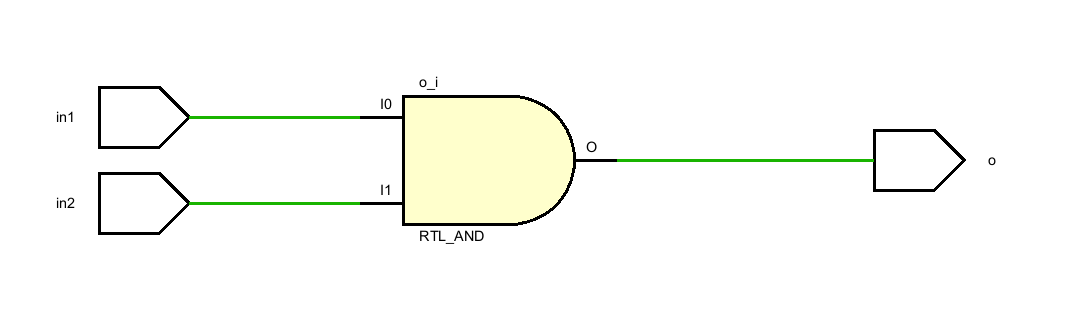
\includegraphics[width=0.8\textwidth]{schematic/and_schematic.png}	
    	\caption{AND gate schematic}
    	\label{AND gate schematic}
    \end{figure}
    
    \begin{figure}[H]
    	\centering
    	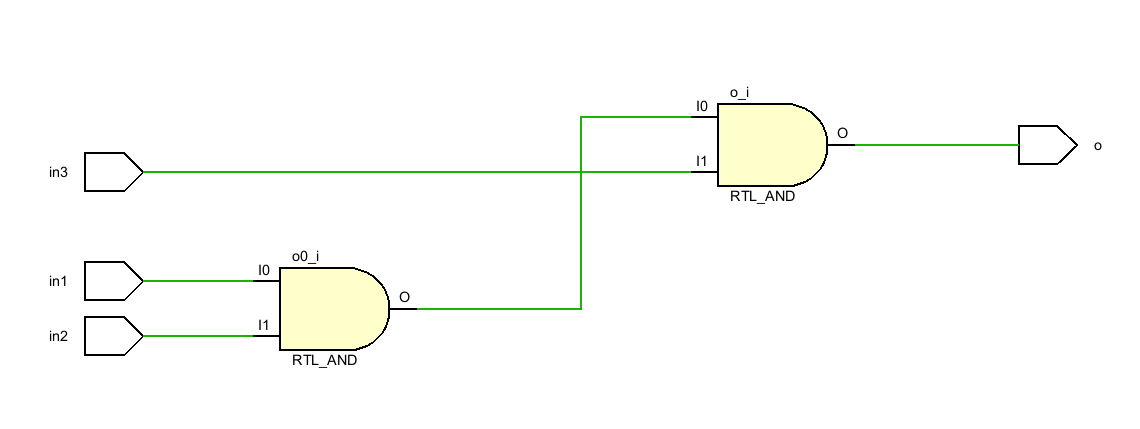
\includegraphics[width=0.8\textwidth]{schematic/three_and_schematic.png}	
    	\caption{3-input AND gate schematic}
    	\label{3-input AND gate schematic}
    \end{figure}
    
    \begin{figure}[H]
    	\centering
    	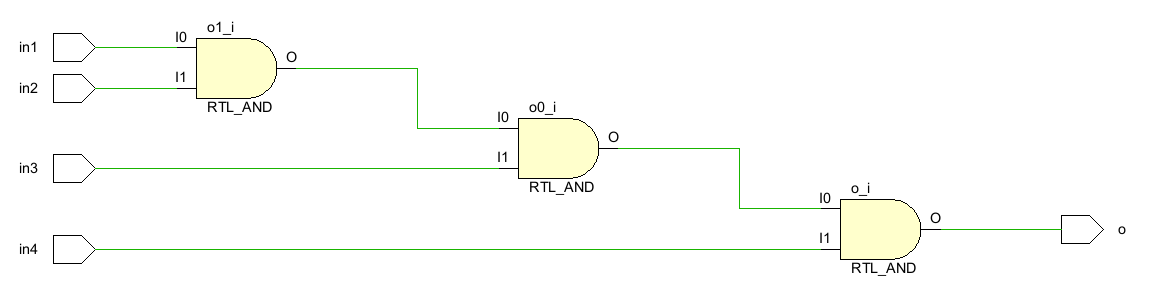
\includegraphics[width=0.8\textwidth]{schematic/four_and_schematic.png}	
    	\caption{4-input AND gate schematic}
    	\label{4-input AND gate schematic}
    \end{figure}
    
    \begin{figure}[H]
    	\centering
    	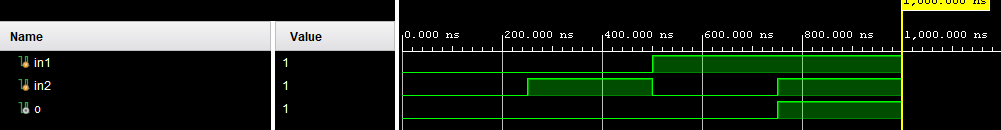
\includegraphics[width=1\textwidth]{simulations/and_sim.png}	
    	\caption{AND gate simulation}
    	\label{AND gate simulation}
    \end{figure}
    
    \begin{figure}[H]
    	\centering
    	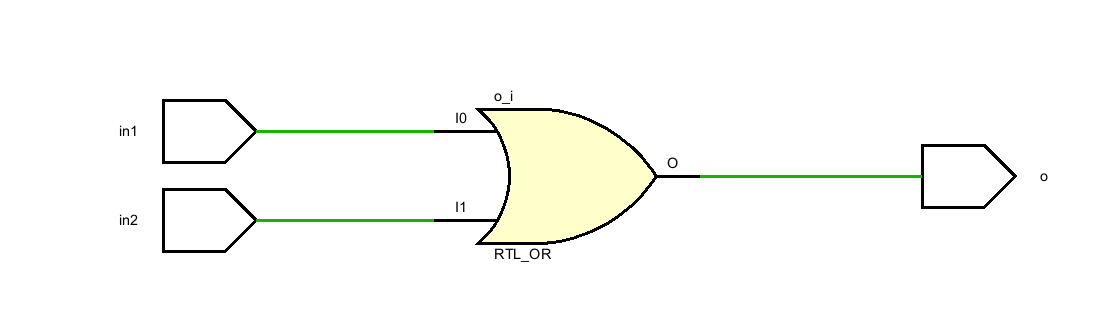
\includegraphics[width=0.8\textwidth]{schematic/or_schematic.png}	
    	\caption{OR gate schematic}
    	\label{OR gate schematic}
    \end{figure}
    
    \begin{figure}[H]
    	\centering
    	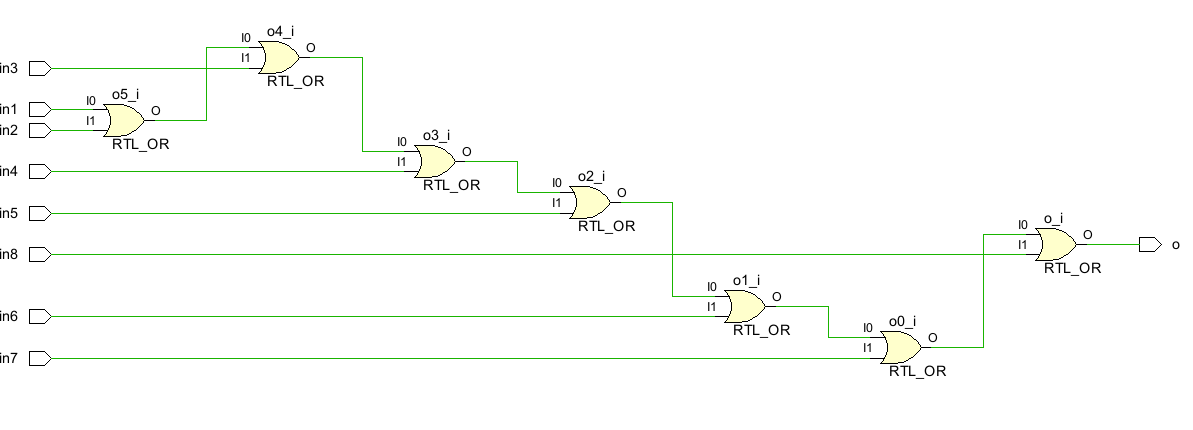
\includegraphics[width=0.8\textwidth]{schematic/8or_schematic.png}	
    	\caption{8-input OR gate schematic}
    	\label{8-input OR gate schematic}
    \end{figure}
    
    \begin{figure}[H]
    	\centering
    	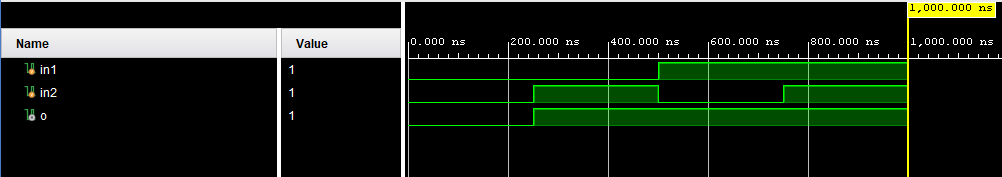
\includegraphics[width=1\textwidth]{simulations/or_sim.png}	
    	\caption{OR gate simulation}
    	\label{OR gate simulation}
    \end{figure}
    
    \begin{figure}[H]
    	\centering
    	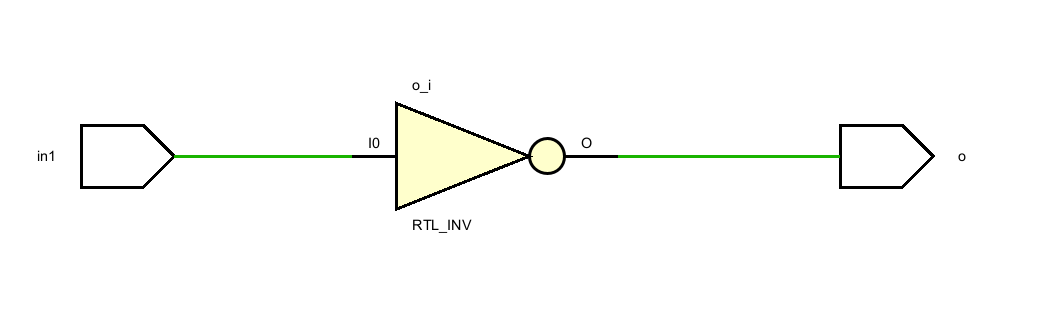
\includegraphics[width=0.8\textwidth]{schematic/not_schematic.png}	
    	\caption{NOT gate schematic}
    	\label{NOT gate schematic}
    \end{figure}
    
    \begin{figure}[H]
    	\centering
    	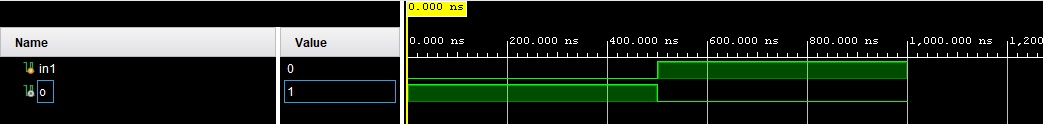
\includegraphics[width=1\textwidth]{simulations/not_sim.png}	
    	\caption{NOT gate simulation}
    	\label{NOT gate simulation}
    \end{figure}
    
    \begin{figure}[H]
    	\centering
    	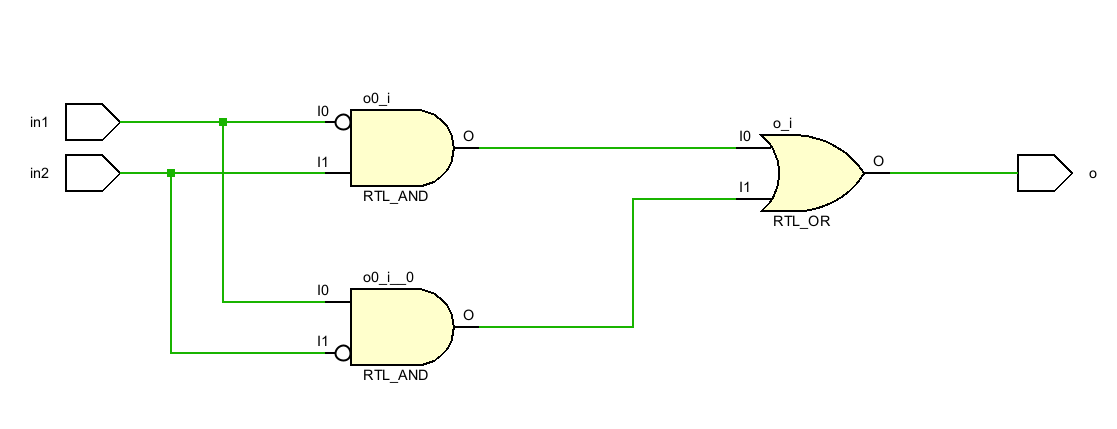
\includegraphics[width=0.8\textwidth]{schematic/xor_schematic.png}	
    	\caption{XOR gate schematic}
    	\label{XOR gate schematic}
    \end{figure}
    
    \begin{figure}[H]
    	\centering
    	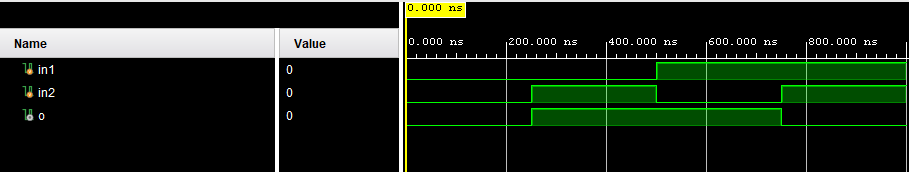
\includegraphics[width=1\textwidth]{simulations/xor_sim.png}	
    	\caption{XOR gate simulation}
    	\label{XOR gate simulation}
    \end{figure}
    
    \begin{figure}[H]
    	\centering
    	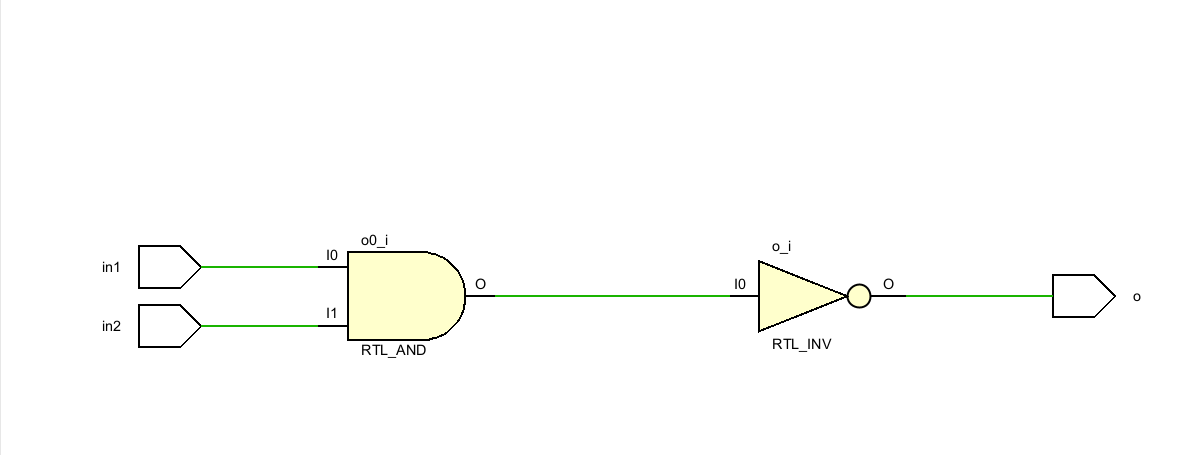
\includegraphics[width=0.8\textwidth]{schematic/nand_schematic.png}	
    	\caption{NAND gate schematic}
    	\label{NAND gate schematic}
    \end{figure}
    
    \begin{figure}[H]
    	\centering
    	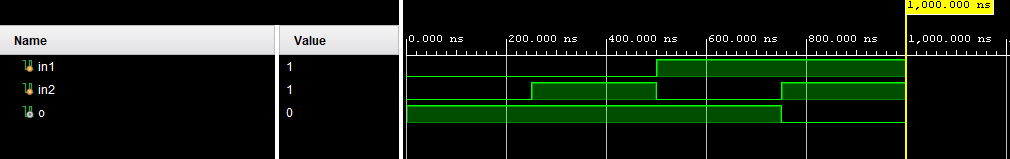
\includegraphics[width=1\textwidth]{simulations/nand_sim.png}	
    	\caption{NAND gate simulation}
    	\label{NAND gate simulation}
    \end{figure}

    \begin{figure}[H]
    	\centering
    	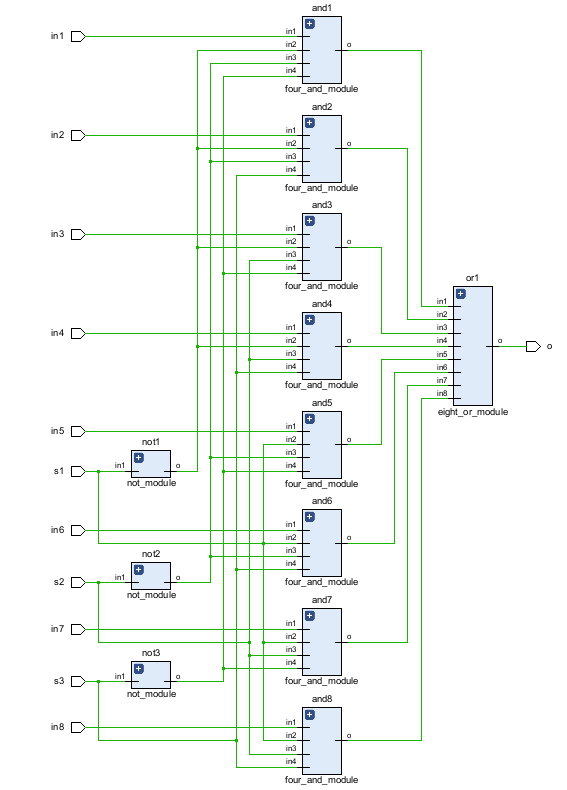
\includegraphics[width=0.8\textwidth]{schematic/mux_schematic.png}	
    	\caption{MUX schematic}
    	\label{MUX schematic}
    \end{figure}
    
    \begin{figure}[H]
    	\centering
    	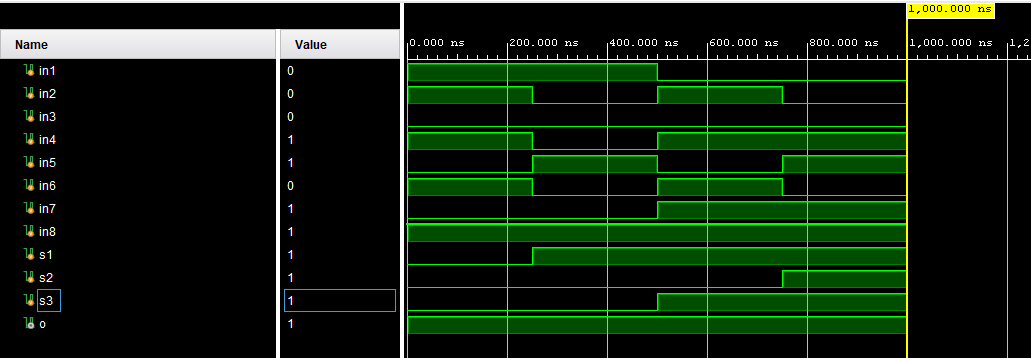
\includegraphics[width=1\textwidth]{simulations/mux_sim.png}	
    	\caption{MUX simulation}
    	\label{MUX simulation}
    \end{figure}

    \begin{figure}[H]
    	\centering
    	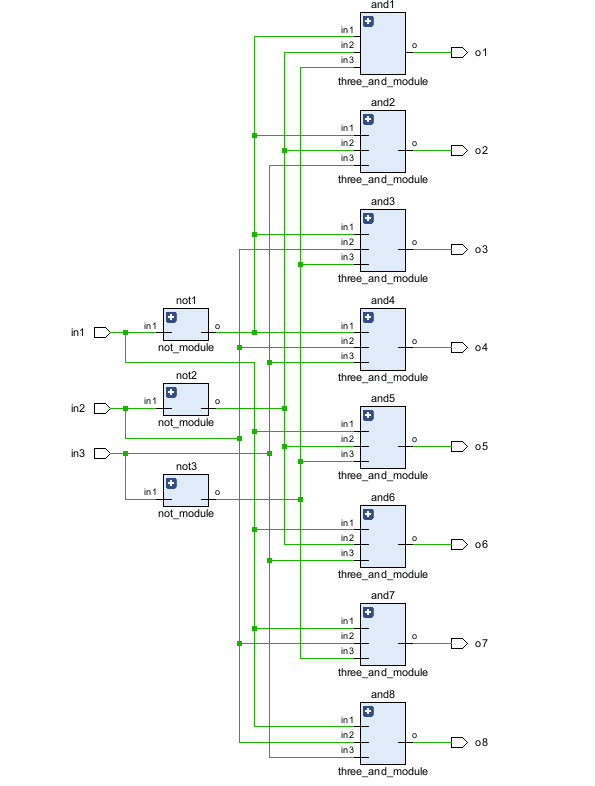
\includegraphics[width=0.8\textwidth]{schematic/decoder_schematic.png}	
    	\caption{decoder schematic}
    	\label{decoder schematic}
    \end{figure}
    
    \begin{figure}[H]
    	\centering
    	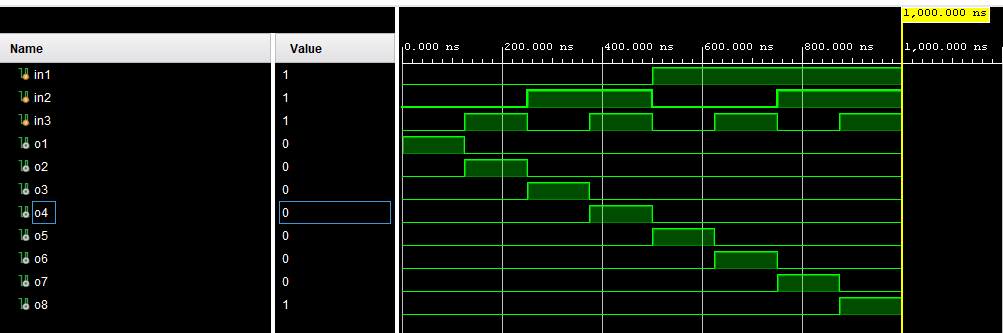
\includegraphics[width=1\textwidth]{simulations/decoder_sim.png}	
    	\caption{decoder simulation}
    	\label{decoder simulation}
    \end{figure}
    
\subsubsection{PART 2}

    \begin{figure}[H]
    	\centering
    	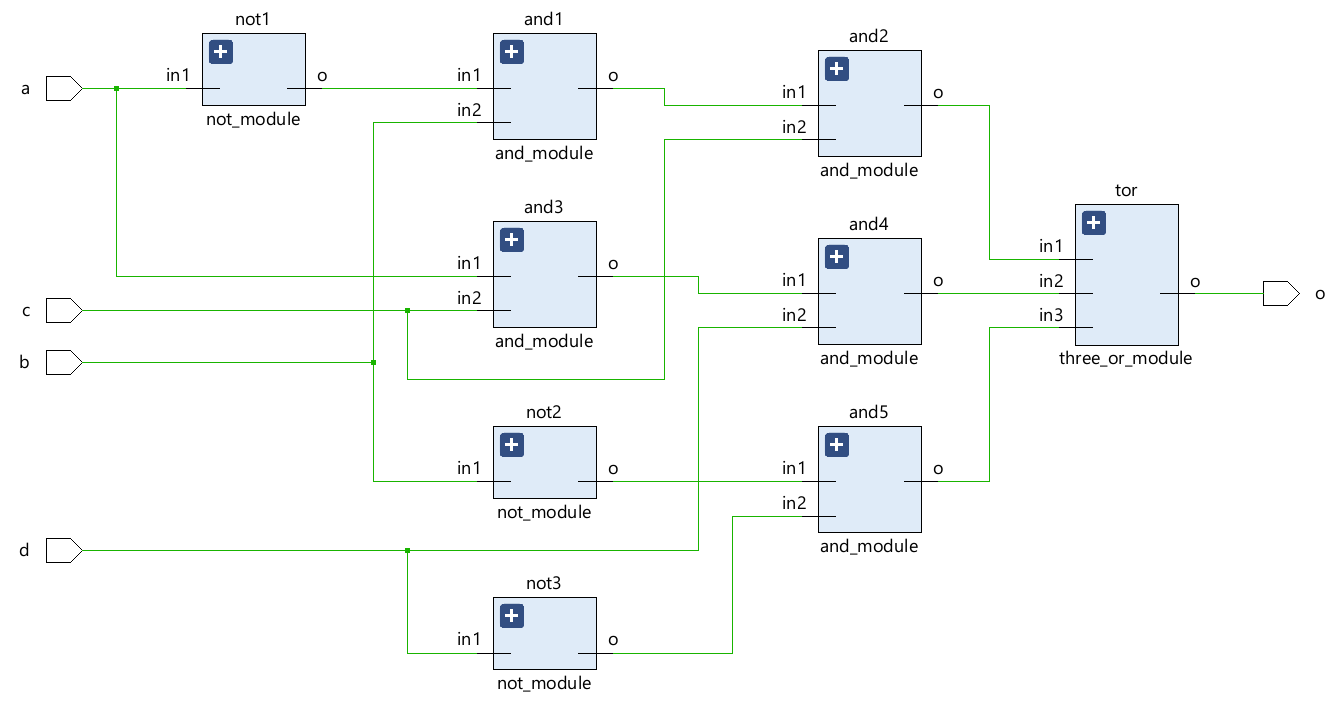
\includegraphics[width=0.8\textwidth]{schematic/prelim_1_d_sch.png}	
    	\caption{preliminary 1 using AND OR NOT gates}
    	\label{preliminary 1 using AND OR NOT gates}
    \end{figure}


    \begin{figure}[H]
    	\centering
    	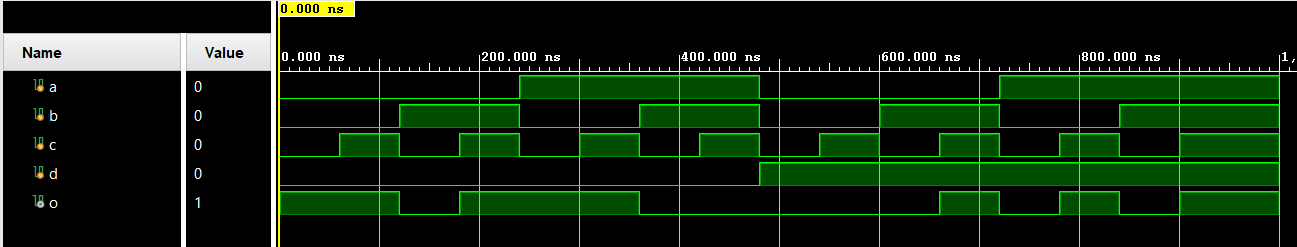
\includegraphics[width=1\textwidth]{simulations/prelim_1_d_result.png}	
    	\caption{results for preliminary 1 using AND OR NOT gates}
    	\label{results for preliminary 1 using AND OR NOT gates}
    \end{figure}



\subsubsection{PART 3}

    \begin{figure}[H]
    	\centering
    	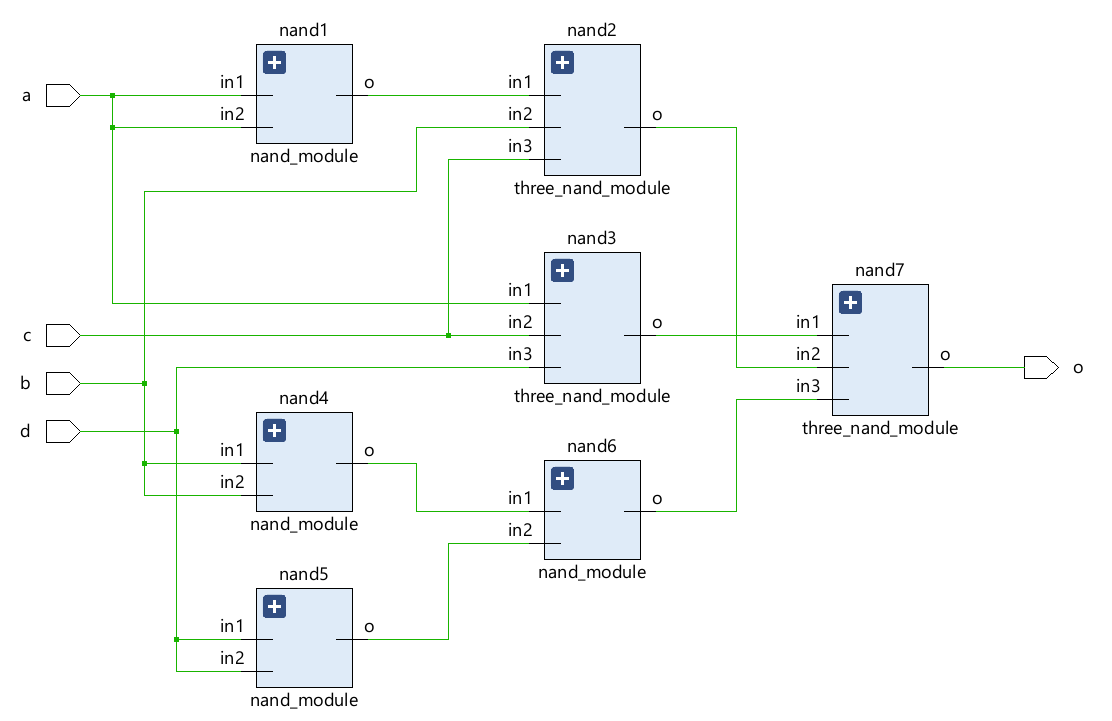
\includegraphics[width=0.8\textwidth]{schematic/prelim_1_e_sch.png}	
    	\caption{preliminary 1 using only NAND gates}
    	\label{preliminary 1 using only NAND gates}
    \end{figure}


    \begin{figure}[H]
    	\centering
    	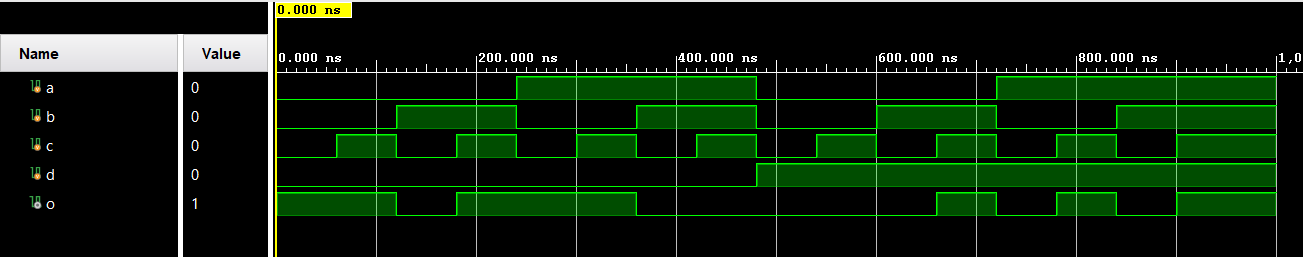
\includegraphics[width=1\textwidth]{simulations/prelim_1_e_result.png}	
    	\caption{results for preliminary 1 using only NAND gates}
    	\label{results for preliminary 1 using only NAND gates}
    \end{figure}




\subsubsection{PART 4}

    \begin{figure}[H]
    	\centering
    	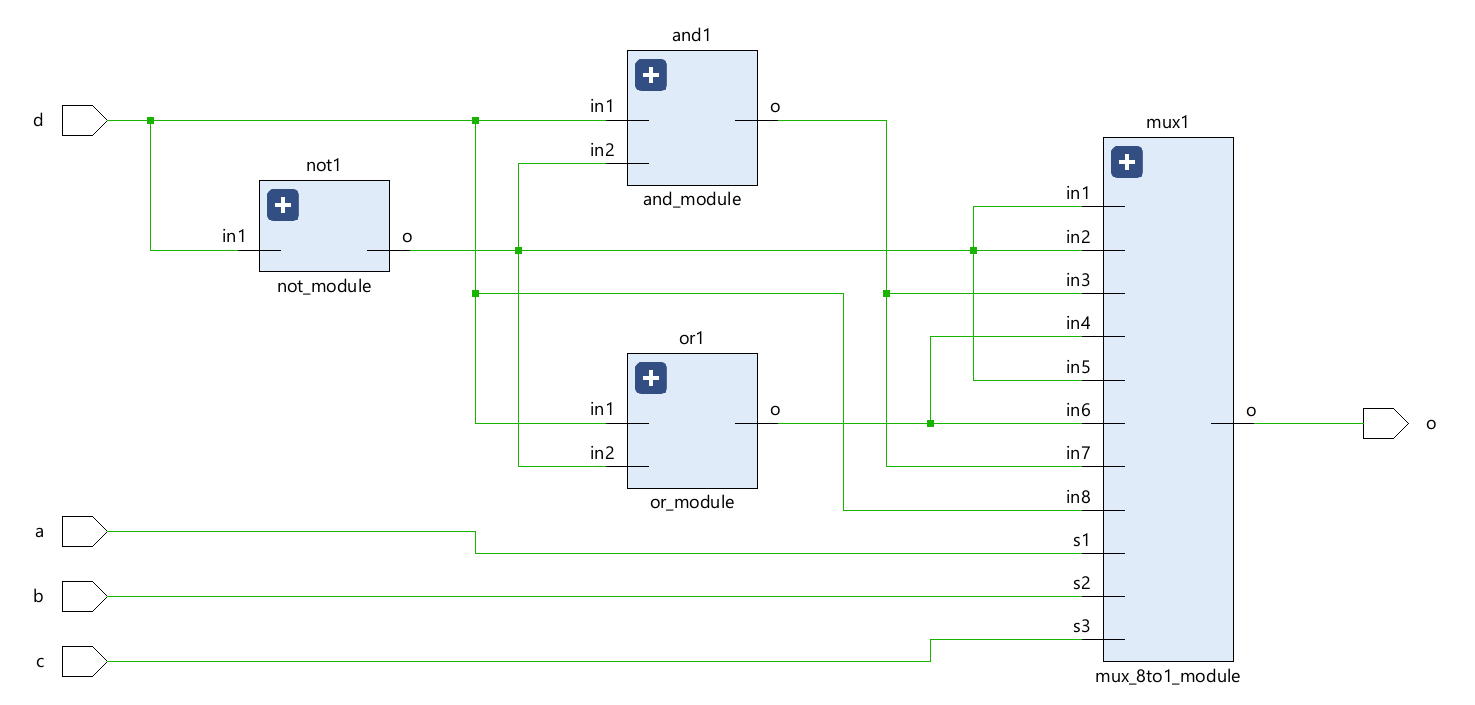
\includegraphics[width=0.8\textwidth]{schematic/prelim_1_f_sch.png}	
    	\caption{preliminary 1 using 8x1 MUX}
    	\label{preliminary 1 using 8x1 MUX}
    \end{figure}


    \begin{figure}[H]
    	\centering
    	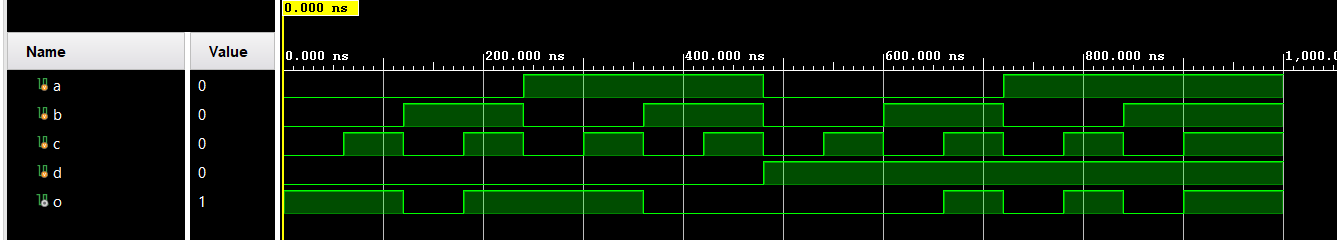
\includegraphics[width=1\textwidth]{simulations/prelim_1_f_result.png}	
    	\caption{results for preliminary 1 using 8x1 MUX}
    	\label{results for preliminary 1 using 8x1 MUX}
    \end{figure}




\subsubsection{PART 5}
    \begin{figure}[H]
    	\centering
    	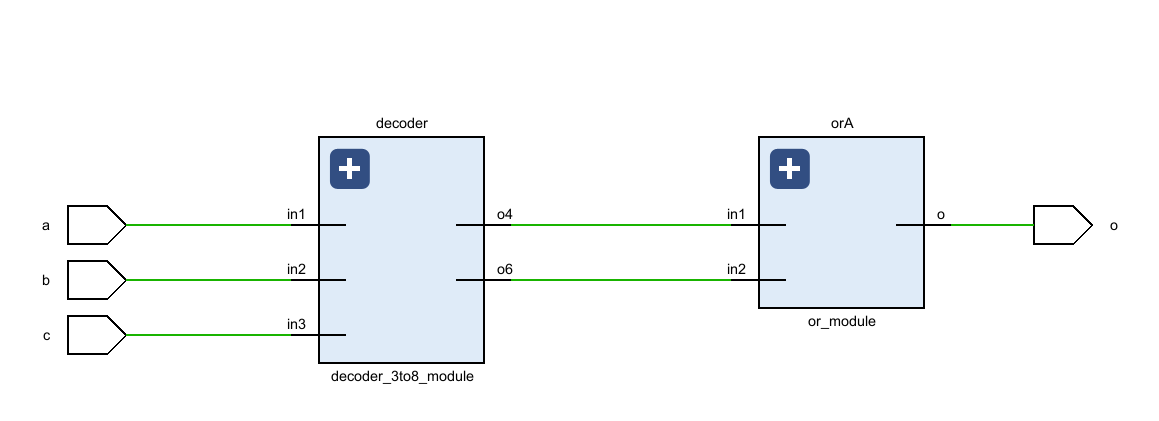
\includegraphics[width=0.8\textwidth]{schematic/F2_schematic.png}	
    	\caption{F2 schematic}
    	\label{F2 schematic}
    \end{figure}
    
    \begin{figure}[H]
    	\centering
    	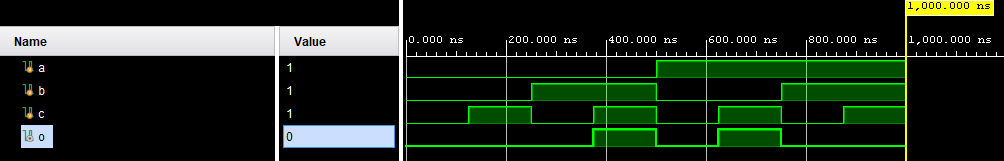
\includegraphics[width=0.8\textwidth]{simulations/F2_sim.png}	
    	\caption{F2 simulation}
    	\label{F2 simulation}
    \end{figure}
    
    \begin{figure}[H]
    	\centering
    	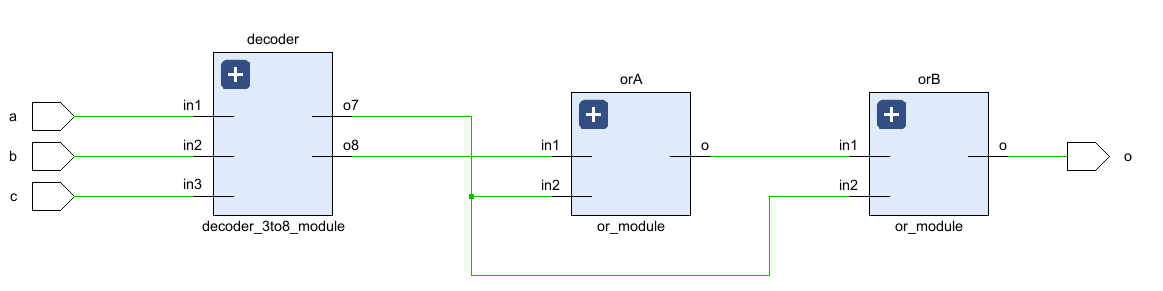
\includegraphics[width=0.8\textwidth]{schematic/F3_schematic.png}	
    	\caption{F3 schematic}
    	\label{F3 schematic}
    \end{figure}
    
    \begin{figure}[H]
    	\centering
    	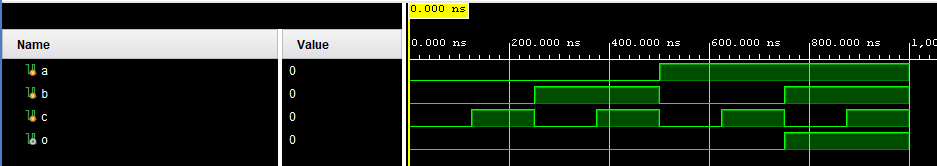
\includegraphics[width=0.8\textwidth]{simulations/F3_sim.png}	
    	\caption{F3 simulation}
    	\label{F3 simulation}
    \end{figure}
\subsubsection{PART 6}
    \begin{figure}[H]
    	\centering
    	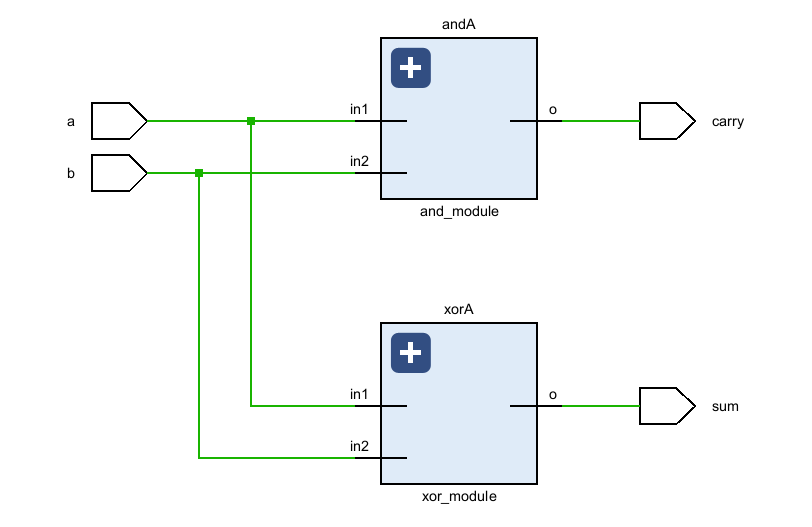
\includegraphics[width=0.8\textwidth]{schematic/half_bit_adder_schem.png}	
    	\caption{1-Bit half adder schematic}
    	\label{1-Bit half adder schematic}
    \end{figure}
    
    \begin{figure}[H]
    	\centering
    	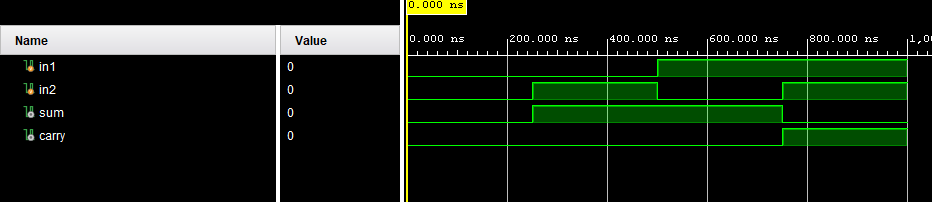
\includegraphics[width=1\textwidth]{simulations/half_bit_adder_sim.png}	
    	\caption{1-Bit half adder simulation}
    	\label{1-Bit half adder simulation}
    \end{figure}
\subsubsection{PART 7}
    \begin{figure}[H]
    	\centering
    	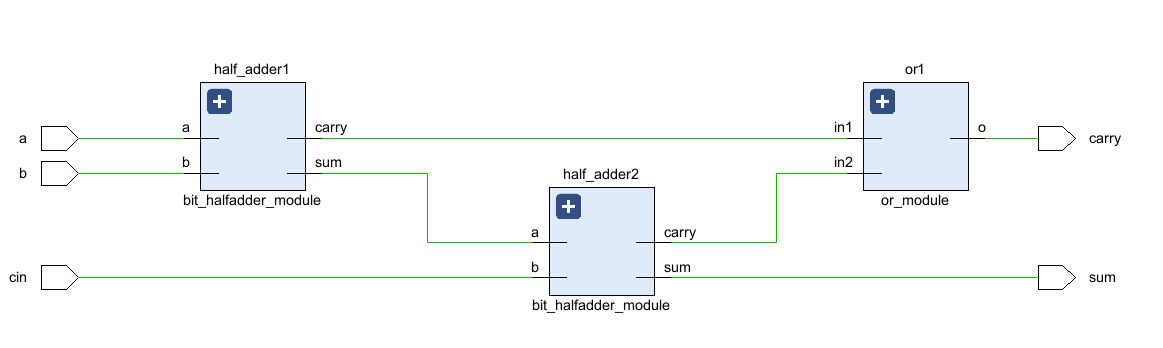
\includegraphics[width=0.8\textwidth]{schematic/1bit_full_adder_schem.png}	
    	\caption{1-bit full adder schematic}
    	\label{1-bit full adder schematic}
    \end{figure}
    
    \begin{figure}[H]
    	\centering
    	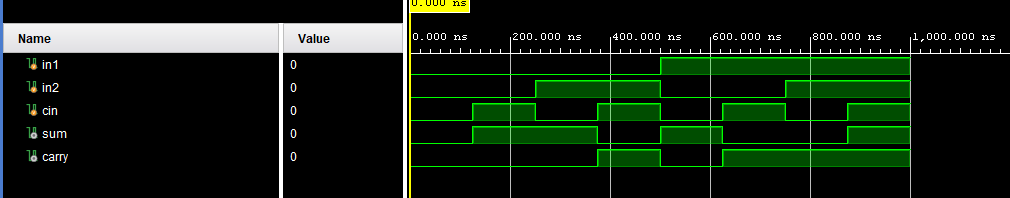
\includegraphics[width=1\textwidth]{simulations/1bit_full_adder_sim.png}	
    	\caption{1-bit full adder simulation}
    	\label{1-bit full adder simulation}
    \end{figure}
\subsubsection{PART 8}
    \begin{figure}[H]
    	\centering
    	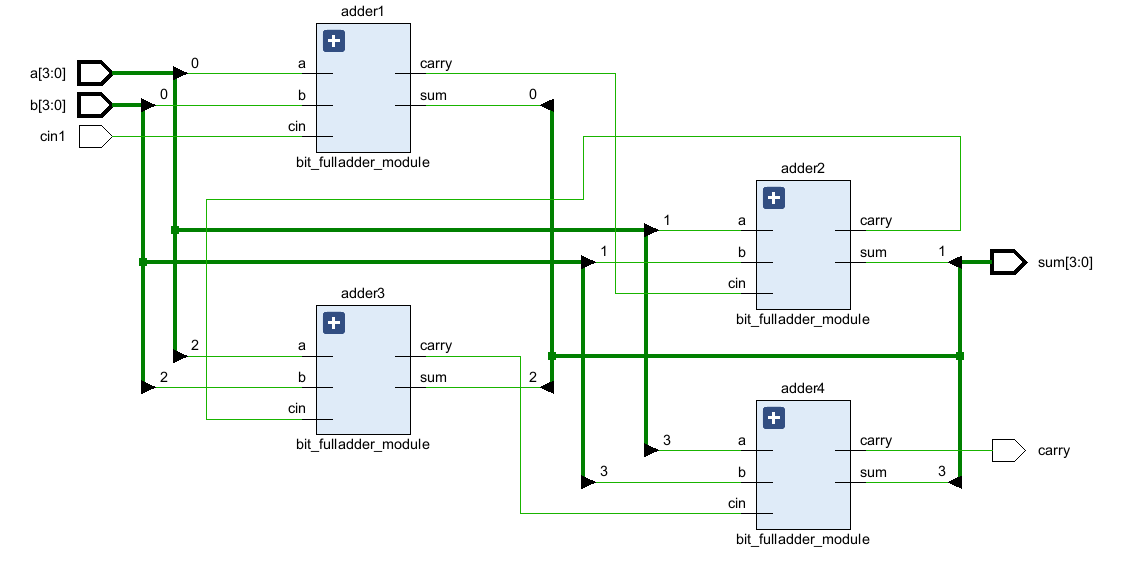
\includegraphics[width=0.8\textwidth]{schematic/4bitadder_schematic.png}	
    	\caption{4-bit full adder schematic}
    	\label{4-bit full adder schematic}
    \end{figure}
    
    \begin{figure}[H]
    	\centering
    	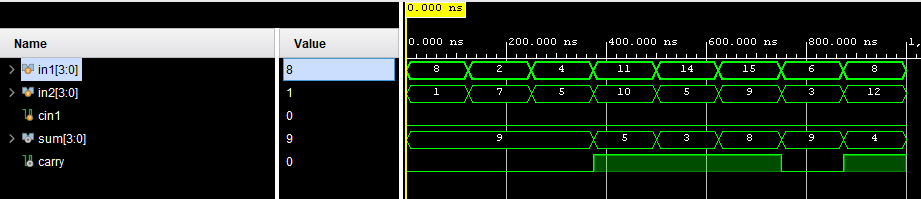
\includegraphics[width=1\textwidth]{simulations/4bitadder_sim.png}	
    	\caption{4-bit full adder simulation}
    	\label{4-bit full adder simulation}
    \end{figure}
\subsubsection{PART 9}
    \begin{figure}[H]
    	\centering
    	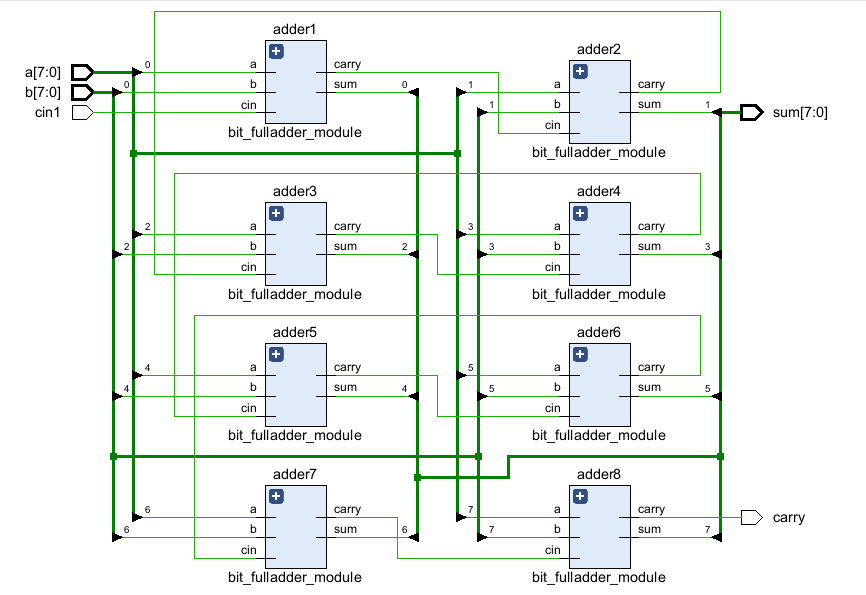
\includegraphics[width=0.8\textwidth]{schematic/8bitadder_schematic.png}	
    	\caption{8-bit full adder schematic}
    	\label{8-bit full adder schematic}
    \end{figure}
    
    \begin{figure}[H]
    	\centering
    	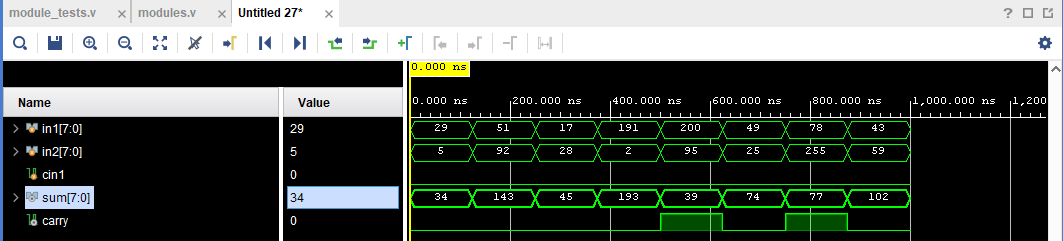
\includegraphics[width=1\textwidth]{simulations/8bitadder_sim.png}	
    	\caption{8-bit full adder simulation}
    	\label{8-bit full adder simulation}
    \end{figure}


    
\subsubsection{PART 10}

\begin{figure}[H]
    	\centering
    	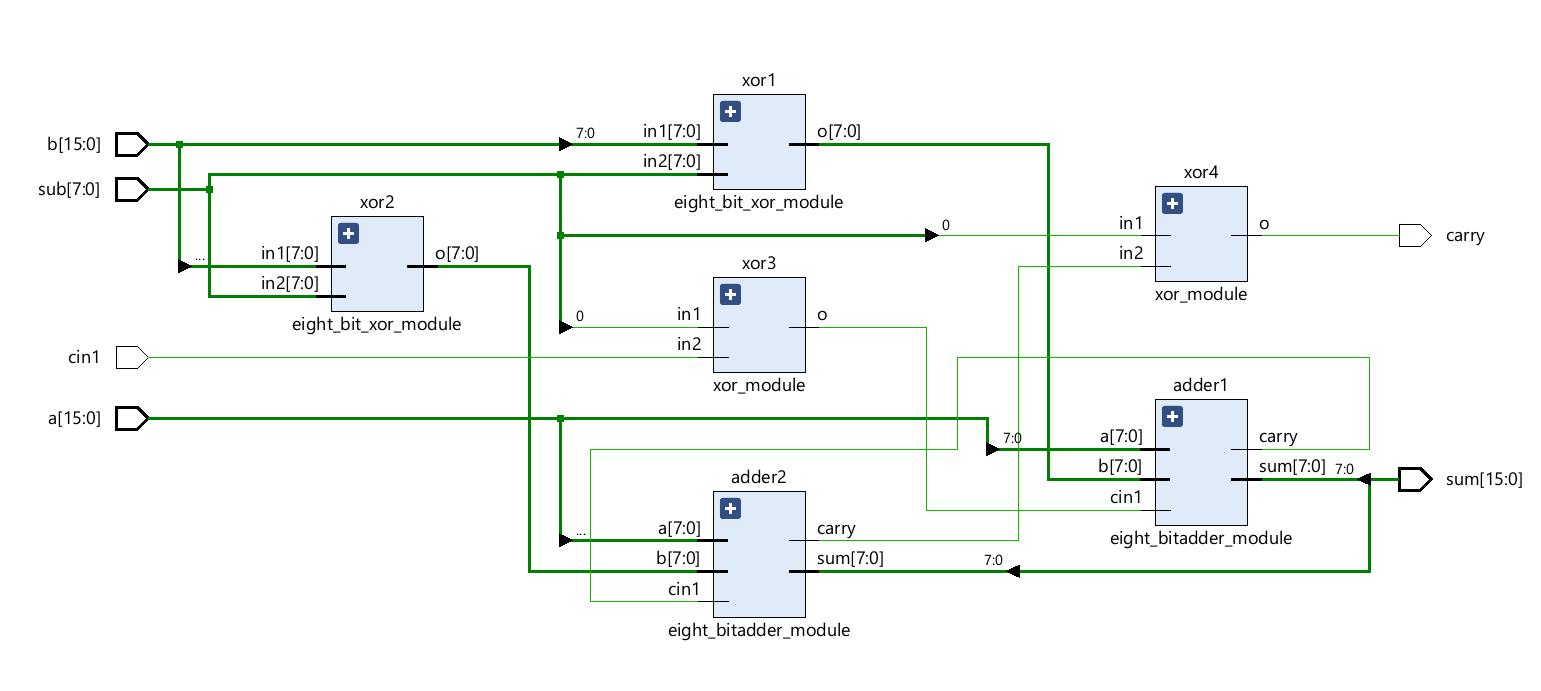
\includegraphics[width=0.8\textwidth]{schematic/part10_sch.png}	
    	\caption{schematic of 16-bit-adder substractor}
    	\label{schematic of 16-bit-adder substractor}
    \end{figure}
    
    \begin{figure}[H]
    	\centering
    	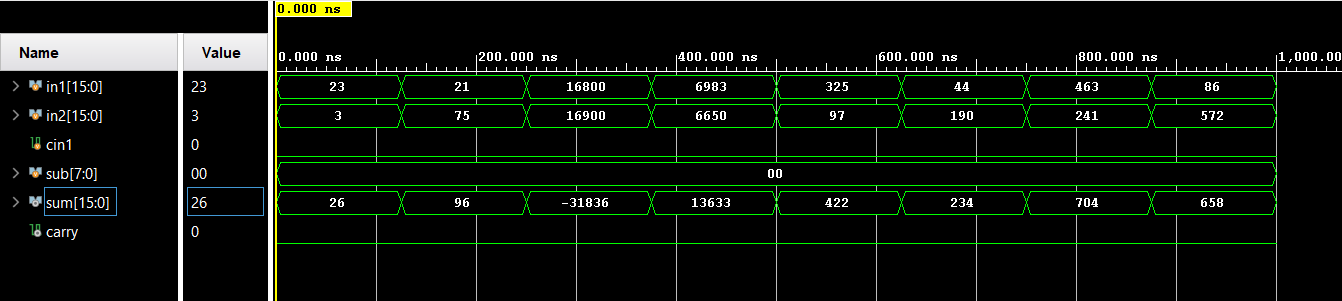
\includegraphics[width=1\textwidth]{simulations/part10_result.png}	
    	\caption{simulation of part 10}
    	\label{simulation of part 10}
    \end{figure}

However, due to the overflow, result of 16800+16900 shows wrongly.

\subsubsection{PART 11}

\begin{figure}[H]
    	\centering
    	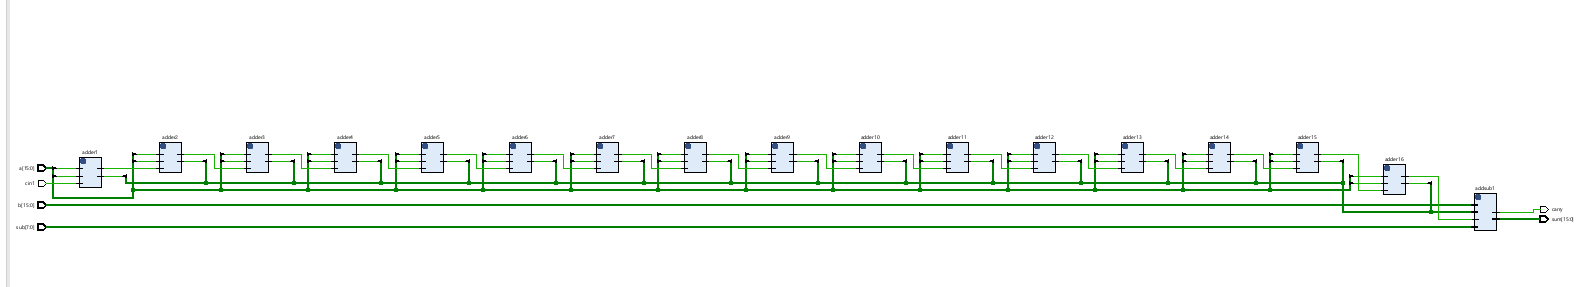
\includegraphics[width=1\textwidth]{schematic/part11_sch.png}	
    	\caption{schematic of B-2A using 16-bit-adder-substractor(rightmost one) \& full adders}
    	\label{schematic of B-2A using 16-bit-adder-substractor(rightmost one) & full adders}
    \end{figure}
    
    \begin{figure}[H]
    	\centering
    	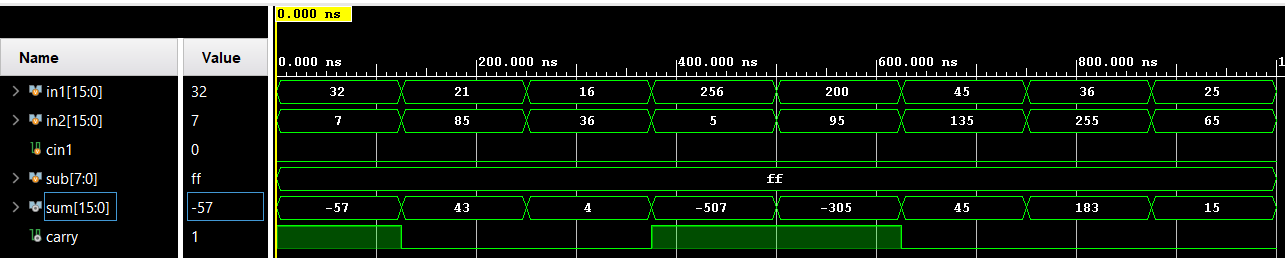
\includegraphics[width=1\textwidth]{simulations/part11_result.png}	
    	\caption{simulation of part 11}
    	\label{simulation of part 11}
    \end{figure}

\subsection{truth tables}

    \begin{figure}[H]
    	\centering
    	\includegraphics[width=0.6\textwidth]{truth tables/and.png}	
    	\caption{and gate truth table}
    	\label{and gate truth table}
    \end{figure}
    
    \begin{figure}[H]
    	\centering
    	\includegraphics[width=0.5\textwidth]{truth tables/or.png}	
    	\caption{or gate truth table}
    	\label{or gate truth table}
    \end{figure}
    
    \begin{figure}[H]
    	\centering
    	\includegraphics[width=0.5\textwidth]{truth tables/not.png}	
    	\caption{not gate truth table}
    	\label{not gate truth table}
    \end{figure}
    
    \begin{figure}[H]
    	\centering
    	\includegraphics[width=0.8\textwidth]{truth tables/xor.png}	
    	\caption{xor gate truth table}
    	\label{xor gate truth table}
    \end{figure}
    
    \begin{figure}[H]
    	\centering
    	\includegraphics[width=0.8\textwidth]{truth tables/nand.png}	
    	\caption{nand gate truth table}
    	\label{nand gate truth table}
    \end{figure}
    
    \begin{figure}[H]
    	\centering
    	\includegraphics[width=0.8\textwidth]{truth tables/mux.png}	
    	\caption{8:1 mux truth table}
    	\label{8:1 mux truth table}
    \end{figure}
    
    \begin{figure}[H]
    	\centering
    	\includegraphics[width=0.8\textwidth]{truth tables/decoder.png}	
    	\caption{3:8 decoder truth table}
    	\label{3:8 decoder truth table}
    \end{figure}
    
    \begin{figure}[H]
    	\centering
    	\includegraphics[width=0.8\textwidth]{truth tables/half.png}	
    	\caption{1-bit half adder truth table}
    	\label{1-bit half adder truth table}
    \end{figure}

    \begin{figure}[H]
    	\centering
    	\includegraphics[width=0.8\textwidth]{truth tables/one.png}	
    	\caption{1-bit full adder truth table}
    	\label{1-bit full adder truth table}
    \end{figure}
    
\pagebreak

\section{CONCLUSION}
With this homework, we learned how to use verilog in different applications. We write modules for NOT, AND, OR, XOR, NAND gates with different input size capabilities and designed 8x1 multiplexer and 3:8 decoder. For summation we designed half 1- bit adder, 1-bit full adder, 4-bit full adder, 8-bit full adder. Not only for summation but also for subtraction, we designed 16-bit adder substractor. We used our designed modules in various application. Such as with given expression we designed implementations with using AND, OR, NOT gates; using only NAND gates and using 8x1 MUX, NOT, AND, OR gates. We made functions with decoders and or gates. At the end, with using 16-bit adders and full-adders we designed implementation for the expression B-2A.



\end{document}

